\subsection{Usability Evaluation} 
\begin{frame}{IDA}{Instant Data Analysis}
	\begin{itemize}
        \item Why IDA?
		\item 3 persons conducting
		\begin{itemize}
            \item 2 taking notes
            \item 1 test monitor
		\end{itemize}
        \item 5 test subjects, experts
		\item Video recorder
		\item Screen recorder
		\item Follow-up questions
	\end{itemize}
    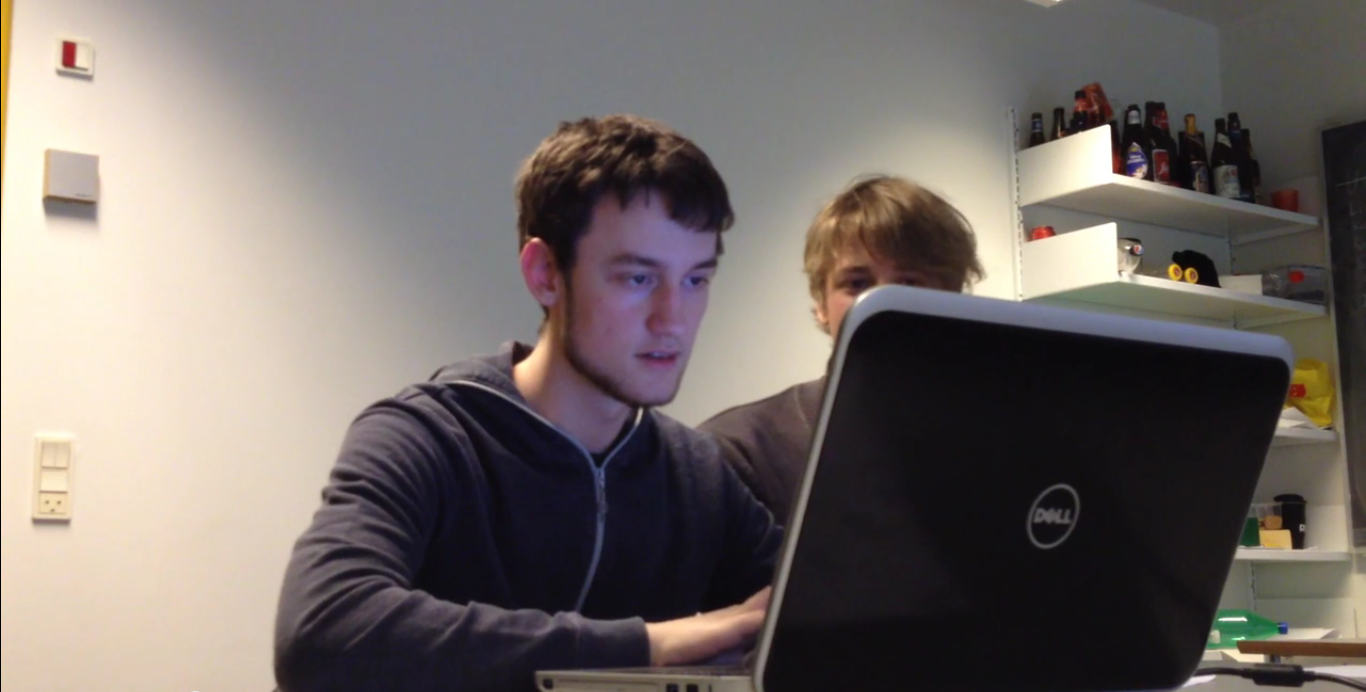
\includegraphics[scale=0.2]{./graphics/UsabilityTest_Screenshot01}
\end{frame}

\begin{frame}{IDA outcome}
    \begin{itemize}
	\item Critical problems
		\begin{itemize}
			\item Scheduled meal page, update button
			\item Deleting meal
			\item Automatic or manual update
		\end{itemize}
	\item Serious problems
		\begin{itemize}
			\item Planning meal the wrong way
			\item Top bar in recipe screen
			\item Changing the number of days to shop for 
		\end{itemize}
	\item Cosmetic problems
		\begin{itemize}
			\item Dividing of setting screen
			\item Adding ingredient to lists
			\item Too specific rating
		\end{itemize}
        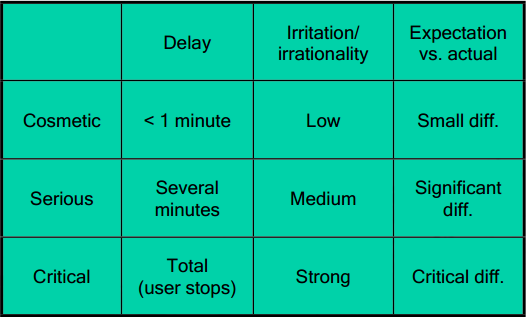
\includegraphics[scale=0.3]{./graphics/UsabilityTest_Screenshot04}
    \end{itemize}
\end{frame}

\begin{frame}{Usability Problems}
    \begin{itemize}
        \item Scheduled meal page, update button (Critical)
        \newline 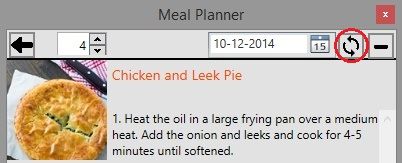
\includegraphics[scale=0.4]{./graphics/UsabilityTest_datepickerRedCircle}
        \item Planning meal the wrong way (Serious)
        \newline 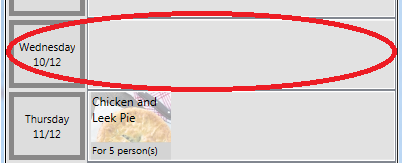
\includegraphics[scale=0.4]{./graphics/UsabilityTest_Screenshot02}
        \item Too specific rating (Cosmetic)
        \newline 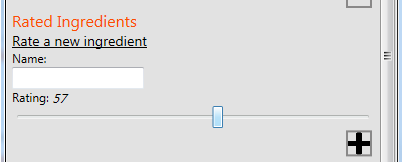
\includegraphics[scale=0.4]{./graphics/UsabilityTest_Screenshot03}
    \end{itemize}
\end{frame}

\begin{frame}{Heuristic Evaluation}{Molich and Nielsen’s 9 heuristics for usability}
    \begin{itemize}
        \item Conducted by us
    \end{itemize}
    \begin{enumerate}
        \item Simple and Natural Dialogue
        \item Speak the User’s Language 
        \item Minimize the User’s Memory Load 
        \item Be Consistent
        \item Provide Feedback 
        \item Provide Clearly Marked Exits 
        \item Provide Shortcuts 
        \item Provide Good Error Messages
        \item Error Prevention
    \end{enumerate}
\end{frame}

\begin{frame}{Waterfall versus Iterative}
	    \centering \fbox{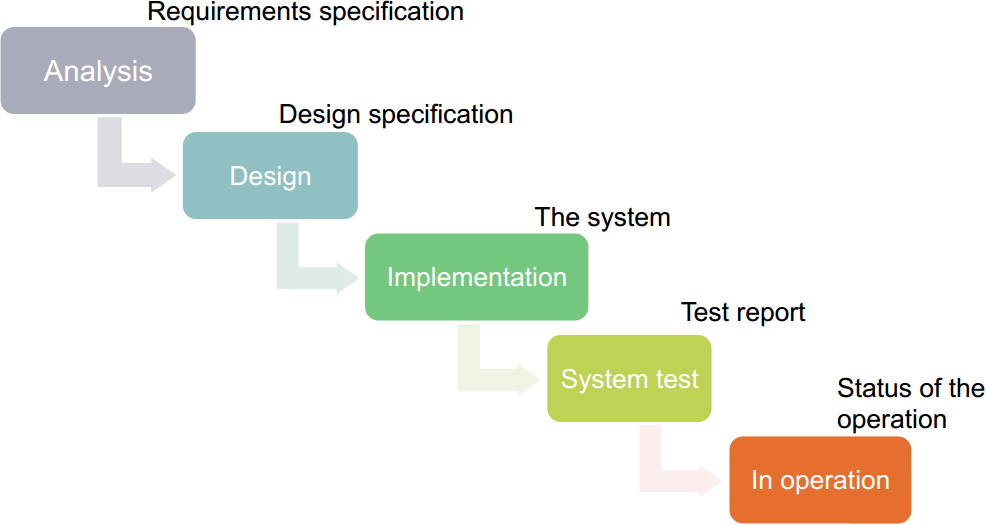
\includegraphics[scale=0.25]{./graphics/UsabilityTest_Waterfall}}
        \newline \centering \fbox{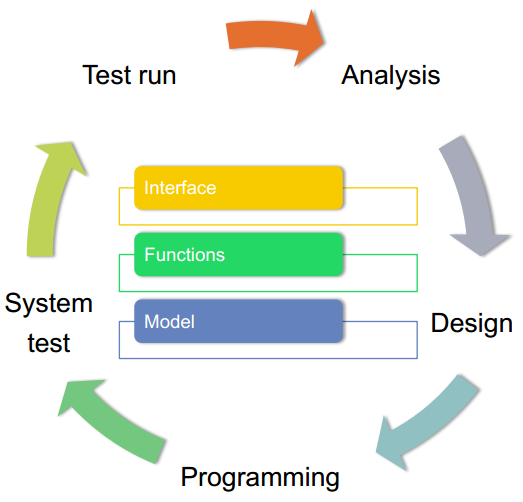
\includegraphics[scale=0.25]{./graphics/UsabilityTest_Iterative}}
\end{frame}